\section{Authorized-grid calibration and fixed-grid relocation}
This section supersedes the calibration completion statements in earlier checkpoints. Earlier experiments are retained separately as historical diagnostics. The present run uses the expanded cohort; integer event identifiers must not be joined to the older 1,003-event cohort.

\paragraph{Reference input and transformation.}
Tan et al.'s distribution at revision \path{f84c9c9d} (full revision in the source receipt) supplies \path{models/3d_vmod}, attributed to Battaglia et al. (2008; doi:10.1111/j.1365-2478.2007.00687.x). The current instruction explicitly permits that file as a starting/reference input. Its unchanged 122,853-byte copy is \path{data/grid_calibration/reference_grid.original}; SHA-256 is \path{dc36fe2a542fc7a3b6c473c48ec109c53ddd77a1721f509b920fea97fb0166f3}. It is not claimed to be an independently retrieved original 2008 array. The grid contains 23 longitude, 14 latitude and 27 depth nodes, ordered longitude fastest, then latitude and depth. Longitude/latitude are degrees east/north, depth is km below sea level, $V_p$ is km/s, and the second volume is dimensionless $V_p/V_s$. Pointwise $V_s=V_p/(V_p/V_s)$. Depth extends from $-0.5$ to a 200 km padding node; the shallow model ends at 7 km. The original article describes an 18 by 18 by 9 km volume with 0.5 km spacing, unlike these irregular/padded axes. The historical transformation remains undocumented. The generic TomoDD reader and manual establish the encoding; the current 3D file is not regridded.

Regional averaging uses explicit assumed boxes: $14.01$--$14.21^\circ$E, $40.76$--$40.87^\circ$N for the caldera and $14.11$--$14.16^\circ$E, $40.80$--$40.84^\circ$N for Pozzuoli--Solfatara. Node weights are $\cos(\mathrm{latitude})$; $V_p$ and pointwise $V_s$ are averaged separately. Exact $V_p=0.1$ km/s nodes are interpreted as nonsolid/air and excluded from the 1D average. The first entirely solid plane, 0.1 km deep, extends upward to $-0.5$ km. Horizontal padding and the terminal 200 km layer are excluded from regional depth integration. These masks, layer boundaries and weights are assumptions where Tan gives region names without numerical masks. They do not recover an undocumented transformation.

\paragraph{Independent observations and corrections to the failed pilot.}
The saved expanded input contains 868 processed files, 26 station names and 8511.520 union channel-hours. Independent association times span 2022-01-21T01:14:48.080 to 2025-03-20T23:58:58.807, with large gaps; this is not full-period coverage. 916 of 1015 associations have positive travel times and no observed nonpositive S--P pairs. Calibration additionally requires at least four P and two S picks, more than ten total picks, gap below $180^\circ$ and no initial 0/8 km depth-bound hit, leaving 38 unreviewed candidates. This is not Tan's manually selected 373-event sample. No routine catalog or author result selects these events.

The first eight-layer attempts produce $V_p\leq V_s$ after the station-delay inversion and are rejected. The generic VELEST guide recommends avoiding low-velocity layers initially, locating events before velocity inversion, merging similar unresolved layers and damping unresolved deep velocities. Accordingly LOWVELOCLAY is zero, prelocation uses 14 iterations, and four layer tops are $-0.5,1,3,5$ km. The deepest velocity damping is 100, other layer damping is 1; deeper unconstrained velocities are not freely fitted. A failed damping-1000 attempt overflowed the fixed-width output field and is retained as a serialization failure. The corrected four-layer run preserves physical ordering. It performs two seven-iteration calibration rounds followed by three declared convergence checks, without changing observations or relaxing the paper's final filters. The reference P delay is fixed at IV.CFB3.. The last-pass model, not the still-moving second-round fit, supplies the catalog run.

\paragraph{Validation and catalog filtering.}
Both regional fits satisfy the stated local stability gates: every horizontal/depth change below 100 m, velocity change below 0.05 km/s, and station-delay change below 0.02 s in the final extra pass. The lower converged unweighted phase RMS is 0.218 s (caldera). These are numerical gates, not absolute accuracy. Regional starts still give maximum differences of 654.7 m horizontally and 1.04 km in depth. Complete 32/64-bit paths differ by 557.8 m horizontally, 0.89 km in depth, 0.32 km/s in velocity and 0.25 s in station delay. Starting both precisions from the same converged fit instead gives identical printed coordinates and velocities. Thus a small final change does not remove path sensitivity; printed equality does not bound unprinted differences. Reviewed phases and independent absolute-location validation remain undone; held-out refitting is reported in the additional validation section. The fit is not accepted as a scientific catalog.

All 916 usable events enter the fixed-model run. Three passes precede $|r|>0.4$ s rejection; another pass precedes $|r|>0.3$ s rejection. The fifth pass and final six-pick, 0.25 s reported-RMS and $300^\circ$ gap filters leave 216 exploratory locations. Fixed models and station corrections were checked after each pass; rejected phases are not replaced. The generic reported event statistic differs from unweighted phase RMS, as verified in the preceding checkpoint.

\paragraph{Observed differential times and TomoDD.}
round 1: 132 outputs, 124 gap passes; round 2: 124 outputs, 123 gap passes. both fixed-grid rounds executed; validation pending. The neighbor graph and windows belong to this expanded event set; no old-cohort waveform cache is reused. Exact measured counts, failed windows, controls and residuals are in \path{data/grid_calibration/merged4/tomodd}. Original absolute picks supply phase-pair times; response-corrected two-second windows supply coherency-weighted delays. Ten nearest neighbors, 1--15 Hz filtering, correlation/coherence at least 0.6, maximum lag 0.25 s, six-phase clustering links, LSQR damping 50 and two four-iteration weight blocks are explicit assumptions where configuration is unpublished. JOINT=0 fixes the 3D grid. A second round rebases travel-time differences to the independently updated origins. Generic method tables required by the solver are separated from the example observations in its distribution. No author-fitted corrections, velocity model or earthquake result is substituted. Available provisional numerical results now populate Figures 2--3, S6--S7, S10--S13; scientific acceptance remains unresolved.

\paragraph{Display verification and scientific boundaries.}
Every current generated figure is rebuilt from saved numerical products by \path{scripts/publication_plots.py}. Input/output hashes and panel correspondence are in \path{data/grid_calibration/style/plot_inventory.json}. Figure S5 uses the printed 0--5 km depth limits and ticks 0,1,2,3,4,5; Figure 1A has printed ticks 0,2,4 but unlabeled endpoints, so 0--5 km is an explicitly approximate normalization rather than an exact recovery. Neither numerical table changes. Magenta denotes depths above 5 km: 4 in 1A and 2 in S5; white is reserved below zero. Missing magnitudes remain crosses. The area law $0.7+3\,10^{M_d-2}$ points squared is a display assumption, not a recovered published formula. S4/S15 do not print a numerical spectral color scale; their disclosed normalized-PSD display is $-80$ to 0 dB, with white/black under/over colors. Counts and ranges are saved in \path{spectral_scales.json}. S2 uses documented instrument classes; no copied relief or elevation colorbar is manufactured. Diagnostic figures have consistent typography but are explicitly not publication figures. Figure 3 now has an explicitly provisional counterpart. Figure 4A--B still lack a returned mechanism; no beachball is invented.

\paragraph{Rebuild and audit trail.}
Run \path{.venv/bin/python scripts/rebuild_grid_workflow.py} from the repository root. It checks the existing independent processing checkpoint, rebuilds generic solvers, regenerates grid-derived starts, executes calibration/validation and both relocation attempts where supported, plots saved data and compiles both PDFs. The saved independent waveform-window cache may be reused only with matching input/output hashes; \path{--remeasure} recomputes it from recordings. The current procedure does not imply that unfinished full-period acquisition or inference was executed. Controls, own serialized inputs, logs and results are preserved in \path{data/grid_calibration/run_records.zip}; machine-readable procedure and scientific outcomes are separate. Earlier models/results remain in Git and their labeled historical directories. The current grid authorization changes input eligibility, not numerical validation requirements.
The generic solver originally overwrote earlier clusters' residual tables. The output-only patch appends every cluster; final gaps now use only stations with positive-weight retained residuals. This correction changes the trial gap-passing counts and supersedes the last-cluster-only diagnostics, which are preserved separately. All 124 final output events have residuals represented. The final per-observation RMS is 0.0430 s for waveform differences and 0.1086 s for picked-phase constraints. Neither value establishes correct event identity or absolute location accuracy.

\begin{figure}[H]\centering
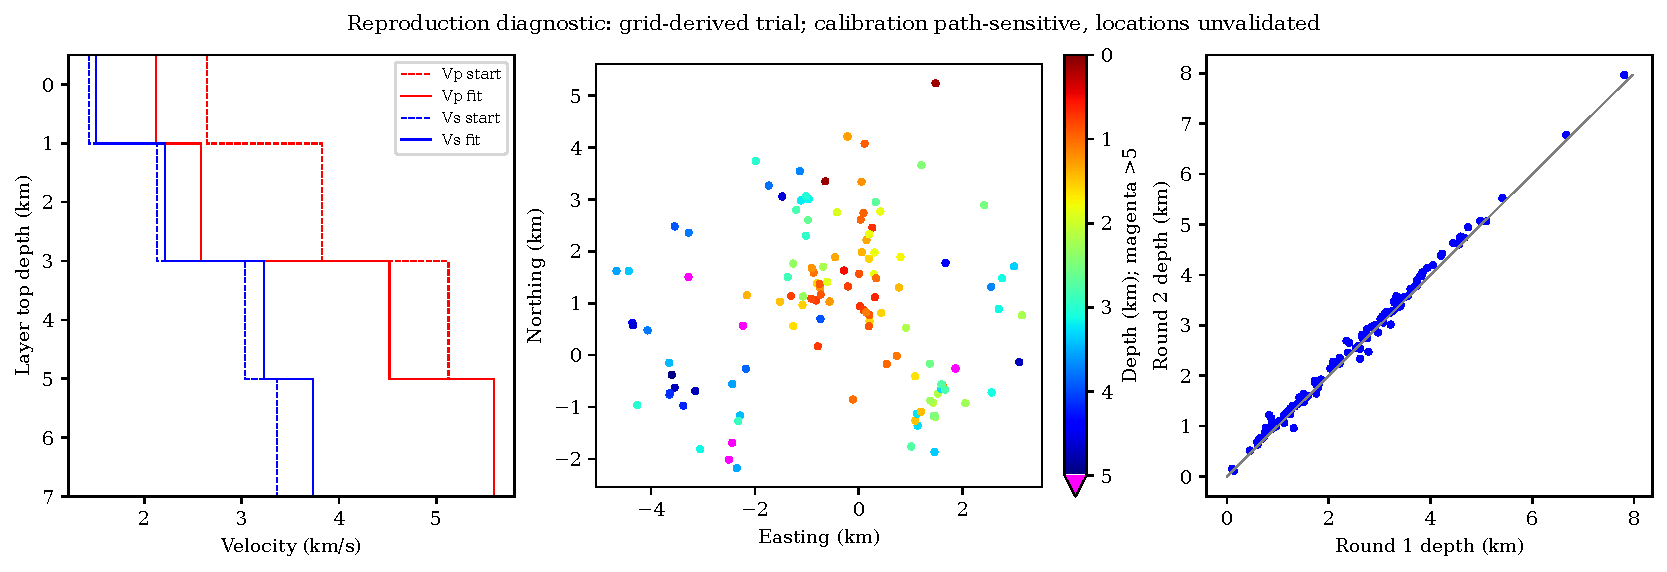
\includegraphics[width=.97\linewidth]{figures/grid_calibration_diagnostic.pdf}
\caption{Reproduction diagnostic, not a publication panel. Grid-derived starting and independently fitted layer velocities, exploratory second-round TomoDD locations and the change in depth between rounds. Fixed color limits are 0--5 km; magenta retains deeper results. Calibration path dependence and unreviewed phases prevent interpreting these patterns as recovered faults.}
\end{figure}
